\section{Feature Extraction from Various Datatypes}

\TD{TODO: Feature Extraction}

\r{representations of the original features}

\r{can bed used to reduce the number of features (effectively dimensionality reduction). However, not always a reduction, in the sense that new feature representations may also be created.}

\subsection{Feature Engineering}

\r{acquisition and/or systematic improvement of features}

\r{TODO: features are learned,not engineered in deep learning models}

% TODO: placement and naming
\subsubsection{Kernel}

\textcolor{blue}{the following can't be separated linearly as is.}

% {{{kernelized_2class4clust_2dimg}}}
\begin{figure}
\centering
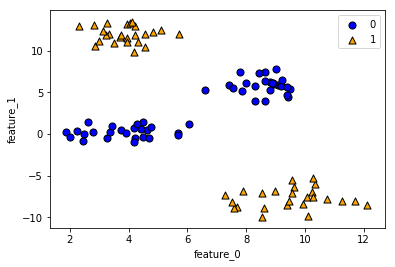
\includegraphics[width=0.65\textwidth]{./sync_imgs/kernelized/2class4clust/2dimg.png}
\label{fig:kernelized_2class4clust_2dimg}
\end{figure}

\r{but what if we produce a new feature (feature 1 ** 2). Adding non-linear features is a powerful method for allowing linear methods to separate non-linear data. However, which features, combinations of features, and types of features is often not easily known. And adding may of these features may become computationally limiting. The {kernel trick}\index{kernel trick} (discussed in more detail in \ref{sec:kernel_trick}) allows for a classifier to learn in a higher-dimensional space, without actually computing these (potentially computationally limiting) representations.}

% {{{kernelized_2class4clust_3dimg}}}
\begin{figure}
\centering
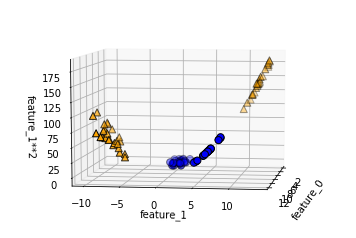
\includegraphics[width=0.65\textwidth]{./sync_imgs/kernelized/2class4clust/3dimg.png}
\label{fig:kernelized_2class4clust_3dimg}
\end{figure}


\subsubsection{Feature Crosses}

% TODO: figure of linearly separable dataset and or a xor dataset
% makes some non-linear problems (xor) linear

\r{combine two or more categorical features. Feature crossing is only possible when working with categorical features. When working with continuous features, the values can be discretized prior to the feature cross}


% how much to translate feature 1 and 2 are parameters that need to be learned
% "discreteize" the input space
% feature crosses "memorize" -- "Memorization works when LOTS of data for a 
% single cell in the input space & the distribution of data is statistically significant."
% not used as often in traditional ML, but powerful on large datasets
% Rome/New york yellow/white Taxi example

\r{number of inputs.}
% example of 24hrs a day, 7 days a week = 168 inputs in a feature cross of the two.
% TF uses a sparse representation for inputs to address this (one hot encoding and feature crosses)
% input will only activate one input at a time, thus the input is very sparse

\r{It is possible that the feature cross may cause the model to overfit the data.}

% TODO: show example of this happening -- X1,X2 (2 blobs ) = good, X1X1,X2X2,X1X2 = overfit

\r{it is possible to look at the relative weights for the inputs and determine how much each feature is contributing to the decision. This can help determine if maybe the features cross isn't necessary -- L1 regularization (see \textcolor{red}{local ref}) may work to zero out this feature as well.}

% TODO: implementation details and choosing the number of hashbuckets.
% if too small, there could be collisions, "rule of thumb" 1/2sqrt(N) and 2N
% trade off is memorization vs sparsity

% adding an embedded layer (real values, learned)
% learns how to ``embedd'' the feature cross in a lower dimesnsional space
% the features learned in embedded features may be useful to other problems from a seperate/maybe related domain
% using learned embeddings in one city for another city on the same types of inputs

\subsection{Images}

\TD{TODO: Images}


\subsubsection{Video}

\TD{TODO: Video}


\subsection{Natural Language}

\TD{TODO: Natural Language}

\subsubsection{Terminology}

\r{A {corpus}\index{corpus} is a collection of documents. {vocabulary}\index{vocabulary} is a corpus's unique words}

\subsubsection{Pre-processing}

\TD{TODO: Pre-processing}

\r{converting all letters to lowercase}

\r{stemming and lemmatization --- Condensing word forms (derived and inflected) into a single feature. These methods are used to reduce the dimensionality of the features space.}

\paragraph{Stop Word Filtering}

\TD{todo: removing words that are common throughout the language as well as potentially to most of the documents in a corpus. Typically stop words do not convey meaning through their meaning, but rather through their grammatical meaning.}

\paragraph{Tokenization}

\r{Tokenization is the process of splitting and grouping characters together into meaningful sequences. \textcolor{red}{If a document is tokenized, the result is a set of tokens (words).} Tokens are not limited to words however, and may also be shorter sequences like punctuation characters and affixes.}

\TD{TODO: Tokenization example}

\paragraph{Lemmatization}

\TD{TODO: Lemmatization. converting words into their base form --- determining the lemma (morphological root) of an inflected word.}

\paragraph{Stemming}

\TD{TODO: Stemming. There exist many stemming algorithms. Stemming removes all character patterns that appear to be affixes to a word. Note: the resulting word may or may not be a valid word e.g. \textcolor{red}{XXXXXXXX}.}

\subparagraph{Porter Stemming}

\subsubsection{Encoding}

\paragraph{Encoding Methods}

\subparagraph{Bag-of-Words}

\r{{bag-of-words}\index{bag-of-words} similar to one-hot-encoding, it encodes words that appear in text as one feature for each word of interest. Does not encode any other information like syntax, grammar, or order of the words.}

\r{Bag-of-Words encodes the corpus's vocabulary as a feature vector to represent each document. The intuition for using bag-of-words is that documents that contain similar words are likely to be similar to one another.}


\paragraph{tf-idf}

\TD{TODO: tf-idf\index{tf-idf} (Eq.\ref{eq:tf_idf_def}) Inverse Document Frequency is a measure of how common/rare a term is in a corpus --- explain importance}

\begin{equation}
{log\frac{N}{1|XXXXXXXXTODOXXXXXXXXXX|}}
\label{eq:tf_idf_def}
\end{equation}

\subsubsection{Embedding}

% TODO: this section may need to be promoted

% an embedding can be created for any categorical column

% ``embeddings cab be thought of as latent features''

% good starting point for number of dimmensions may be cube root of the possible values

\textcolor{blue}{Embeddings are }

\subparagraph{glove}

\TD{TODO: glove}

\subparagraph{word2vec}

\TD{TODO: word2vec}

\subsubsection{Other Notes}

% 'hashing trick' --- see p59 of Mastering ML with SKL

\subsection{Audio}


\textcolor{green}{TODO: Audio}
